\documentclass[class=report,crop=false]{standalone}
\usepackage[screen]{../exo7book}

\begin{document}

%====================================================================
\chapitre{Représentation des nombres}
%====================================================================

\insertvideo{gyaIXFH5y5I}{partie 1. Représentation des nombres entiers en base $2$}

\insertvideo{qTu_XJ8QNu4}{partie 2. Le binaire en \Python}

\insertvideo{pH0chgSDVIU}{partie 3. Les bases $8$ et $16$}


\lstset{
  language=Python,
  upquote=true,
  columns=flexible,
  keepspaces=true,
  basicstyle=\ttfamily,
  commentstyle=\color{gray},
  keywordstyle=\color{blue},
  %emph={bin,oct,hex},
  emphstyle=\color{blue},
  stringstyle=\color{Green4},
  frame=single,  
  showspaces=false,
  showstringspaces=false,
  literate={>>>}{\textcolor{red}{>\,\!>\,\!>}}{3},
}

%\mdtheorem[style=algostyle]{algo}{Algorihme}
%\renewcommand\thealgo{} % No numeratotion to algo


\subsection*{Objectifs}

\begin{itemize}
\item Savoir ce que sont les représentations de nombres entiers en base $2$, $8$  et $16$.
\item Savoir convertir un nombre entier dans l'une de ces bases.
\item Savoir calculer l'entier connaissant sa représentation dans l'une de ces bases.
\item Connaître les fonctions de \Python\ permettant ces conversions.
\item Savoir les programmer.
\end{itemize}


%%%%%%%%%%%%%%%%%%%%%%%%%%%%%%%%%%%%%%%%%%%%%%%%%%%%%%%%%%%%%%%%
\section{Représentation des nombres entiers en base $2$}


%----------------------------------------------------
\subsection{Motivation}

L'histoire révèle que selon les époques et les lieux, l'écriture des
nombres s'est effectuée de plusieurs façons. Par exemple, le nombre
quarante-sept peut s'écrire :

\begin{itemize}
\item avec des petits traits :
\textbar{}\textbar{}\textbar{}\textbar{}\textbar{} \textbar{}\textbar{}\textbar{}\textbar{}\textbar{} \textbar{}\textbar{}\textbar{}\textbar{}\textbar{} \textbar{}\textbar{}\textbar{}\textbar{}\textbar{} \textbar{}\textbar{}\textbar{}\textbar{}\textbar{} \textbar{}\textbar{}\textbar{}\textbar{}\textbar{} \textbar{}\textbar{}\textbar{}\textbar{}\textbar{} \textbar{}\textbar{}\textbar{}\textbar{}\textbar{} \textbar{}\textbar{}\textbar{}\textbar{}\textbar{} \textbar{}\textbar{} ;
\item avec la numération romaine : \codeinline{XLVII} ;
\item avec la numération de position en utilisant les $10$ chiffres arabes :
  \codeinline{47}.
\end{itemize}

Un système d'écriture des nombres se décrit toujours en précisant les
symboles utilisés (l'alphabet) et les règles d'association de ces
symboles.

Ainsi dans notre système de numération décimale, l'alphabet est
constitué de dix symboles : les dix chiffres $0$, $1$, $2$, $3$, $4$, $5$, $6$, $7$, $8$
et $9$. À l'aide de ces dix symboles, on peut écrire n'importe quel nombre
entier. Le nombre quarante-sept s'écrit $47$ en base $10$ ce qui signifie
que ce nombre est égal à $4\times 10^1 + 7\times 10^0$. De même le
nombre $3010$ s'écrit ainsi parce que
$3010 = 3\times 10^3 + 0\times 10^2 + 1\times 10^1 + 0\times 10^0$.

L'écriture décimale d'un nombre entier est tout simplement une
juxtaposition d'un nombre fini des dix chiffres décimaux, tout comme un
mot s'écrit en juxtaposant les lettres de l'alphabet latin (si on écrit
dans une langue utilisant l'alphabet latin).

L'écriture décimale des nombres convient tout à fait aux humains, mais
moins pour les machines.



En 1645, Blaise Pascal a construit une machine à calculer mécanique, la
pascaline, dans laquelle les nombre sont représentés en base $10$. De
telles machines ont continué à exister jusqu'au XXème siècle.
Mais les ordinateurs sont des machines dans lesquelles les engrenages et
roues dentées ont laissé la place à des transistors : ce sont des
machines électroniques. Les états des dispositifs élémentaires sont
représentés par des tensions électriques. Et il est plus facile de
distinguer deux états (par exemple $5$ volts ou $0$ volts, selon que le courant passe ou pas) 
que $10$ états. On comprend
alors que la représentation décimale des nombres n'est pas la plus
appropriée pour de telles machines. Le binaire avec ses deux symboles
leur convient mieux.

\begin{center}
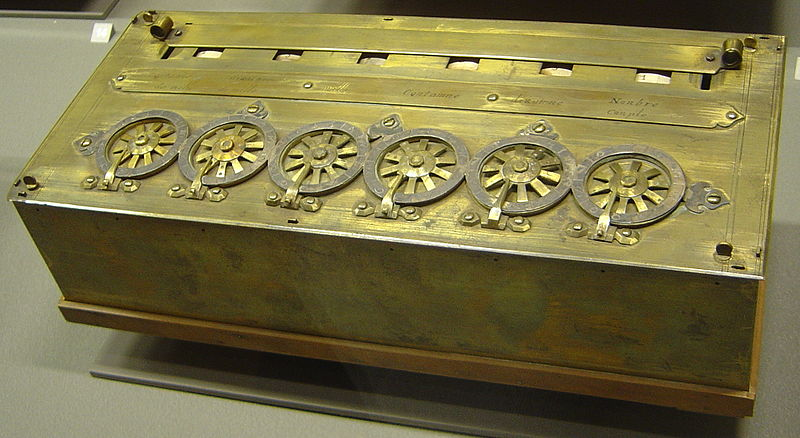
\includegraphics[scale=0.4]{Pascaline.jpg}

{La Pascaline (source Wikipedia)}
\end{center}

%----------------------------------------------------
\subsection{Les puissances de $2$}

Si en base $10$, ce sont les puissances de $10$ ($1$, $10$, $100$, $1000$,...)
qui déterminent l'écriture
d'un nombre, en base $2$, ce sont les puissances de $2$. La table 
donne les premières puissances de deux.

\begin{center}
\begin{tabular}{cc}
$n$&$2^n$\\\hline
0&1\\
1&2\\
2&4\\
3&8\\
4&16\\
5&32\\
6&64\\
7&128\\
8&256\\
9&512\\
10&1024\\
11&2048\\
12&4096\\
13&8192\\
14&16384\\
15&32768\\
16&65536\\
17&131072\\
18&262144\\
19&524288\\
20&1048576
\end{tabular}
\end{center}

%----------------------------------------------------
\subsection{\'Ecriture binaire}

\mybox{
Tout nombre entier admet une unique décomposition en somme de puissances
de $2$.}

L'écriture binaire d'un nombre entier s'appuie sur la décomposition de
cet entier en somme de puissances de $2$ distinctes. Voici ce qu'il en est
pour $47$ et $3010$.


$$47 = 32 + 8 + 4 + 2 + 1 = 2^5 + 2^3 + 2^2 + 2^1 + 2^0
= {\color{red}1}\times 2^5 
+ {\color{red}0}\times 2^4
+ {\color{red}1}\times 2^3 
+ {\color{red}1}\times 2^2 
+ {\color{red}1}\times 2^1 
+ {\color{red}1}\times 2^0.$$

 En utilisant les deux chiffres $0$ et $1$, 
ce nombre s'écrit donc en binaire :
$$47 = \overline{{\color{red}\mathtt{101111}}}_2.$$




Pour $3010$ :
$$
\begin{array}{rcl}
3010 
  &=& 2048 + 512 + 256 + 128 + 64 + 2\\
  &=& {\color{red}1}\times 2^{11}
+ {\color{red}0}\times 2^{10}
+ {\color{red}1}\times 2^9 
+ {\color{red}1}\times 2^8 
+ {\color{red}1}\times 2^7 
+ {\color{red}1}\times 2^6
+ {\color{red}0}\times 2^5
+ {\color{red}0}\times 2^4
+ {\color{red}0}\times 2^3
+ {\color{red}0}\times 2^2
+ {\color{red}1}\times 2^1
+ {\color{red}0}\times 2^0
.
\end{array}
$$
Ainsi :
$3010 = \overline{{\color{red}\mathtt{101111000010}}}_2$.

\bigskip



Voici les écritures binaires des entiers de $0$ à $7$.

\begin{center}
\begin{tabular}{rr}
$0$ & $\overline{\mathtt{0}}_2$ \\
$1$ & $\overline{\mathtt{1}}_2$ \\
$2$ & $\overline{\mathtt{10}}_2$ \\
$3$ & $\overline{\mathtt{11}}_2$ \\
$4$ & $\overline{\mathtt{100}}_2$ \\
$5$ & $\overline{\mathtt{101}}_2$ \\
$6$ & $\overline{\mathtt{110}}_2$ \\
$7$ & $\overline{\mathtt{111}}_2$ \\
\end{tabular}
\end{center}

%----------------------------------------------------
\subsection{Bits et octets}


Les chiffres binaires $0$ et $1$ sont appelés \defi{bits}. Ce mot est la
contraction de l'expression anglaise \emph{binary digit}.
Les entiers de $0$ à $7$ sont les huit seuls entiers qui peuvent s'écrire en
binaire avec trois bits seulement (en complétant par des bits nuls à
gauche si nécessaire).

Un \defi{octet} est un nombre qu'on peut écrire en binaire sur huit
bits. Ce sont les entiers compris entre $0$ et $255$. Ils sont au nombre de
$256$.


\textbf{Warning!}
Le mot anglais \emph{byte} désigne ce qu'en français on nomme octet.
Donc byte $\neq$ bit.



%----------------------------------------------------
\subsection{Mesures de quantité de mémoire}

Longtemps les préfixes \emph{kilo}, \emph{méga}, \ldots{}, appliqués aux
octets pour mesurer des tailles de mémoire désignaient des puissances de
$2$. Or pour toute autre mesure dans le système international, ces mêmes
préfixes désignent des puissances de $10$. 
Une partie de la confusion vient que $2^{10}=1024$ est proche de $1000$.
Pour remédier à cela, la commission électronique 
internationale (IEC) a spécifié de nouveaux
préfixes pour les puissances de $2$.

\begin{center}
\begin{tabular}{llllll}
Nom&Puissance&Abbréviation&Nom&Puissance&Abbréviation\\
\hline
kilooctet&$10^3$&ko&kibioctet&$2^{10}$&Kio\\
megaoctet&$10^6$&Mo&mébioctet&$2^{20}$&Mio\\
gigaoctet&$10^9$&Go&gibioctet&$2^{30}$&Gio\\
téraoctet&$10^{12}$&To&tébioctet&$2^{40}$&Tio\\
pétaoctet&$10^{15}$&Po&pébioctet&$2^{50}$&Pio
\end{tabular}
\end{center}


%%%%%%%%%%%%%%%%%%%%%%%%%%%%%%%%%%%%%%%%%%%%%%%%%%%%%%%%%%%%%%%%
\section{Le binaire en \Python}

%----------------------------------------------------
\subsection{Le binaire en \Python}

La fonction \codeinline{bin} de \Python\ donne une chaîne de caractères
représentant l'écriture binaire de l'entier passé en paramètre. Voici ce
que donne l'aide sur cette fonction :

\begin{lstlisting}
>>> help(bin)
Help on built-in function bin in module builtins:

bin(...)
    bin(number) -> string

    Return the binary representation of an integer.  
\end{lstlisting}

L'aide nous informe que cette fonction prend un nombre entier en
paramètre et renvoie une chaîne de caractères représentant l'écriture
binaire de cet entier.

Appliquons cette fonction à nos deux entiers $47$ et $3010$ :

\begin{lstlisting}
>>> bin(47)
'0b101111'
>>> bin(3010)
'0b101111000010'  
\end{lstlisting}

Nous retrouvons bien l'écriture obtenue plus haut.
À noter que la chaîne de caractères débute par \codeinline{0b}, le
\codeinline{b} mettant en évidence qu'il s'agit de l'écriture binaire d'un
entier.

Pour les nombres négatifs, la représentation binaire est tout simplement
précédée du signe \codeinline{-}, comme on peut le voir sur l'exemple
ci-dessous :

\begin{lstlisting}
>>> bin(-47)
'-0b101111'  
\end{lstlisting}

Jusqu'à présent, nous avons écrit les nombres entiers comme nous avons
l'habitude de le faire usuellement : en base $10$. Mais ceci n'est pas une
nécessité. En \Python\ on peut écrire les nombres entiers directement en
binaire. Il suffit pour cela de faire précéder cette écriture par
\codeinline{0b}.

\begin{lstlisting}
>>> 0b101
5
>>> 0b101 + 47
52 
\end{lstlisting}




\begin{remarque*}
Voici une utilisation ``tautologiques'' de la fonction \codeinline{bin} :
\begin{lstlisting}
>>> bin(0b1011)
'0b1011'
\end{lstlisting} 
Vous remarquerez la présence des simples guillemets autour de la valeur
renvoyée par \codeinline{bin} qui montre bien que cette valeur est une
chaîne de caractères (type \codeinline{str}), alors que l'argument est un
entier (type \codeinline{int}).

\begin{lstlisting}
>>> type(0b110011)
<class 'int'>
>>> type(bin(0b110011))
<class 'str'> 
\end{lstlisting} 
\end{remarque*}



%----------------------------------------------------
\subsection{Algorithme de calcul de l'écriture binaire d'un entier}

Nous avons vu que l'écriture binaire d'un entier s'obtient par la
décomposition de cet entier en somme de puissances de $2$. Mais comment
obtenir cette décomposition ? Doit-on connaître toutes les puissances de
$2$, ou bien disposer une table de ces puissances ? On va voir qu'il n'en
est rien.

Un algorithme simple consiste à diviser cet entier $n$ par deux : on
obtient un quotient $q_1$ et un reste $r_0$ compris entre $0$ et $1$. Puis
on remplace l'entier $n$ par le quotient $q_1$ qu'on divise par deux
pour obtenir un nouveau quotient $q_2$ et un nouveau reste $r_1$ lui
aussi compris entre $0$ et $1$. Et on continue comme cela jusqu'à obtenir un
quotient nul $q_t=0$ et un dernier reste $r_{t-1}$. L'écriture binaire
de $n$ s'obtient en alignant de droite à gauche tous les restes
$r_0, r_1, \ldots r_{t-1}$.

Voici cet algorithme illustré pour $n = 47$.

\begin{itemize}
\item On divise $n$ par $2$, $47 = 2\times 23 + 1$, et on obtient $q_1=23$ et $r_0={\color{red}1}$.
\item On divise $q_1$ par $2$, $23 = 2\times 11 + 1$, et on obtient $q_2=11$ et $r_1={\color{red}1}$.
\item On divise $q_2$ par $2$, $11 = 2\times 5 + 1$, et on obtient $q_3=5$ et $r_2={\color{red}1}$.
\item On divise $q_3$ par $2$, $5 = 2\times 2 + 1$, et on obtient $q_4=2$ et $r_3={\color{red}1}$.
\item On divise $q_4$ par $2$, $2 = 2\times 1 + 0$, et on obtient $q_5=1$ et $r_4={\color{red}0}$.
\item On divise $q_5$ par $2$, $1 = 2\times 0 + 1$, et on obtient $q_6=0$ et $r_5={\color{red}1}$.
\end{itemize}

En six divisions, on arrive à un quotient nul. L'écriture binaire de $n=47$ est donc :
\[47 = \overline{r_{5}r_{4}r_{3}r_{2}r_{1}r_{0}}_2 = \overline{{\color{red}\mathtt{101111}}}_2.\]

Cet algorithme est formalisé avec une boucle tant que dans
l'algorithme de conversion en binaire.

\begin{algo}[\codeinline{en\_bin}. Calcul de l’écriture binaire d’un entier naturel non nul]

\textbf{Entrée :} $n\in\mathbb{N}$ un entier non nul

\textbf{Sortie :} $r_{t-1}r_{t-2}\ldots r_1r_0$ écriture binaire de $n$


\begin{enumerate}
\item $i \leftarrow 0$
\item $q_i \leftarrow n$
\item \textbf{Tant que} $q_i \neq 0$
\item $\qquad q_{i+1} \leftarrow q_i\div 2$
\item $\qquad r_i \leftarrow q_i \pmod{2}$
\item $\qquad i \leftarrow i + 1$
\item \textbf{Fin Tant que}
\item \textbf{Renvoyer :} $r_{i-1}r_{i-2}\ldots r_1r_0$
\end{enumerate}
\end{algo}



\textbf{Note.}
On peut arrêter l'itération dans l'algorithme dès que le dernier
quotient calculé est inférieur à $2$, car on est alors assuré que le
prochain sera nul. On gagne ainsi une division.


%----------------------------------------------------
\subsection{Algorithme de calcul d'un entier représenté en binaire}


Inversement, connaissant l'écriture binaire d'un entier, comment
calculer la valeur de l'entier écrit ?

Bien sûr une solution consiste à développer le calcul d'une somme de
puissances de $2$. Par exemple, avec $n = \overline{{\color{red}\mathtt{101111}}}_2$,
on aurait à calculer

\[\begin{array}{rcl}
n &=& 
{\color{red}1}\times 2^5 
+ {\color{red}0}\times 2^4 
+ {\color{red}1}\times 2^3 
+ {\color{red}1}\times 2^2 
+ {\color{red}1}\times 2^1 
+ {\color{red}1}\times 2^0\\
&=& 32 + 8 + 4 + 2 + 1\\
&=& 47.
\end{array}\]

Cette façon de procéder nécessite le calcul des puissances de $2$
consécutives. Mais, une simple astuce permet de se dispenser du calcul
de ces puissances. Reprenons l'exemple ci-dessus, et effectuons une 
succession de factorisations :
\[\begin{array}{rcl}
n &=& 1\times 2^5 + 0\times 2^4 + 1\times 2^3 + 1\times 2^2 + 1\times 2^1 + 1\times 2^0\\
&=& (1\times 2^4 + 0\times 2^3 + 1\times 2^2 + 1\times 2^1 + 1)\times 2 + 1\\
&=& ((1\times 2^3 + 0\times 2^2 + 1\times 2^1 + 1)\times 2 + 1)\times 2 + 1\\
&=& (((1\times 2^2 + 0\times 2^1 + 1)\times 2 + 1)\times 2 + 1)\times 2 + 1\\
&=& (((({\color{red}1}\times 2 + {\color{red}0})\times 2 + {\color{red}1})\times 2 + {\color{red}1})\times 2 + {\color{red}1})\times 2 + {\color{red}1} \\
&=& 47 \\
\end{array}\]

Dans la dernière ligne, n'apparaissent que :
\begin{enumerate}
\item les bits $r_5r_4r_3r_2r_1r_0$ de l'écriture binaire de $n$,
\item des additions et des multiplications par $2$.
\end{enumerate}

Pas besoin de connaître les puissances de $2$. De plus le nombre de
multiplications par $2$ est égal au nombre de bits de $n$ diminué de $1$.

Cette façon de calculer l'entier correspondant à une écriture binaire
est formalisée dans l'algorithme ci-dessous. C'est
un cas particulier d'un algorithme connu sous le nom d'algorithme de Horner.

\begin{algo}[\codeinline{bin\_2\_dec}. Calcul de l’entier correspondant à une écriture binaire]

\textbf{Entrée :} $r_{t-1}r_{t-2}\ldots r_1r_0$ l'écriture binaire d'un entier $n$

\textbf{Sortie :} valeur de $n$

\begin{enumerate}

\item $n\leftarrow r_{t-1}$ (le bit le plus à gauche dans l'écriture binaire)
\item \textbf{Pour} $i$ variant de $t-2$ à 0 (en décroissant)
\item $\qquad n\leftarrow n\times 2 + r_{i}$
\item \textbf{Fin pour}
\item \textbf{Renvoyer :} $n$
\end{enumerate}
\end{algo}


%%%%%%%%%%%%%%%%%%%%%%%%%%%%%%%%%%%%%%%%%%%%%%%%%%%%%%%%%%%%%%%%
\section{Les bases $8$ et $16$}


Les écritures décimales et binaires des nombres entiers ne sont pas les
seules utilisées. En informatique deux autres bases sont plus ou moins
fréquemment employées :
\begin{itemize}
\item la base $8$ utilisant les huit chiffres de \codeinline{0} à \codeinline{7} ; on
  parle alors d'écriture \defi{octale} des nombres ;
\item la base $16$ utilisant les dix chiffres usuels de \codeinline{0} à
  \codeinline{9} et les six premières lettres de l'alphabet de \codeinline{A} à
  \codeinline{F} ; on parle alors d'écriture \defi{hexadécimale} des
  nombres.
\end{itemize}

%----------------------------------------------------
\subsection{L'octal}

Déterminons les écritures octales des nombres $47$ et $3010$. Pour cela il
suffit d'écrire chacun de ces deux nombres comme somme de puissances de
8. Une méthode pour le faire est de diviser le nombre à écrire par la
base autant de fois que nécessaire.

\begin{itemize}
\item Pour $47$
  \[\begin{array}{rcl}
  47 &=& 8\times 5 + 7\\
  5  &=& 8\times 0 + 5.
  \end{array}\]

  En prenant les restes successifs des divisions qui précèdent, on
  trouve $47 = 5\times 8^1 + 7\times 8^0$. D'où l'écriture octale de $47$:
  \[47 = \overline{\mathtt{57}}_8.\]
\item Pour $3010$
  \[\begin{array}{rcl}
  3010 &=& 8\times 376 + 2\\
  376  &=& 8\times 47 + 0\\
  47   &=& 8\times 5 + 7\\
  5    &=& 8\times 0 + 5.
  \end{array}\]

  En prenant les restes successifs des divisions qui précèdent, on
  trouve $3010 = 5\times 8^3 + 7\times 8^2 + 0\times 8^1 + 2\times 8^0$.
  D'où l'écriture octale de $3010$ :

  \[3010 = \overline{\mathtt{5702}}_8.\]
\end{itemize}

 \bigskip
 
\evidence{Les nombres de 0 à 20 en octal}

 
  
  \begin{center}
    \begin{tabular}[ht]{rrp{2cm}rr}
      0 & $\overline{0}_{8}$ & &10 & $\overline{12}_{8}$\\
      1 & $\overline{1}_{8}$ & &11 & $\overline{13}_{8}$\\
      2 & $\overline{2}_{8}$ & &12 & $\overline{14}_{8}$\\
      3 & $\overline{3}_{8}$ & &13 & $\overline{15}_{8}$\\
      4 & $\overline{4}_{8}$ & &14 & $\overline{16}_{8}$\\
      5 & $\overline{5}_{8}$ & &15 & $\overline{17}_{8}$\\
      6 & $\overline{6}_{8}$ & &16 & $\overline{20}_{8}$\\
      7 & $\overline{7}_{8}$ & &17 & $\overline{21}_{8}$\\
      8 & $\overline{10}_{8}$ & &18 & $\overline{22}_{8}$\\
      9 & $\overline{11}_{8}$ & &19 & $\overline{23}_{8}$\\
      &  & &20 & $\overline{24}_{8}$\\
    \end{tabular}
  \end{center}


L'analogue de la fonction \codeinline{bin} en \Python\ pour l'octal est la
fonction \codeinline{oct}.
\begin{lstlisting}
>>> oct(47)
'0o57'
>>> oct(3010)
'0o5702'
>>> oct(-3010)
'-0o5702'  
\end{lstlisting}

Comme on peut le constater sur ces quelques exemples, la fonction
\codeinline{oct} renvoie une chaîne de caractères préfixées par \codeinline{0o}
ou \codeinline{-0o} selon le signe pour signifier qu'il s'agit bien d'une
écriture octale des nombres.

On peut aussi entrer directement des nombres en les écrivant en base $8$
en les préfixant du \codeinline{0o} :
\begin{lstlisting}
>>> 0o57
47
>>> 2 * 0o57 
94 
\end{lstlisting}

%----------------------------------------------------
\subsection{L'hexadécimal}

Déterminons les écritures hexadécimales des nombres $47$ et $3010$. Pour
cela il suffit d'écrire chacun de ces deux nombres comme somme de
puissances de $16$ avec la technique des divisions successives :

\begin{itemize}
\item Pour $47$

  \[\begin{array}{rcl}
  47 &=& 16\times 2 + 15\\
  2  &=& 16\times 0 + 2.
  \end{array}\]

  En prenant les restes successifs des divisions qui précèdent, on
  trouve $47 = 2\times 16^1 + 15\times 16^0$. D'où l'écriture
  hexadécimale de $47$ en employant le chiffre \codeinline{F} pour représenter
  $15$ :

  \[47 = \overline{\mathtt{2F}}_{16}.\]
\item Pour $3010$

  \[\begin{array}{rcl}
  3010 &=& 16\times 188 + 2\\
  188  &=& 16\times 11 + 12\\
  11   &=& 16\times 0 + 11.
  \end{array}\]

  En prenant les restes successifs des divisions qui précèdent, on
  trouve $3010 = 11\times 16^2 + 12\times 16^1 + 2\times 16^0$. D'où
  l'écriture hexadécimale de $3010$ en utilisant le chiffre \codeinline{B}
  pour $11$, et le chiffre \codeinline{C} pour $12$ :

  \[3010 = \overline{\mathtt{BC2}}_{16}.\]
\end{itemize}

  \bigskip
  
  \evidence{Les nombres de 0 à 20 en hexadécimal}


  
  \begin{center}
    \begin{tabular}[ht]{rrp{2cm}rr}
      0 & $\overline{0}_{16}$ & &10 & $\overline{\mathtt{A}}_{16}$\\
      1 & $\overline{1}_{16}$ & &11 & $\overline{\mathtt{B}}_{16}$\\
      2 & $\overline{2}_{16}$ & &12 & $\overline{\mathtt{C}}_{16}$\\
      3 & $\overline{3}_{16}$ & &13 & $\overline{\mathtt{D}}_{16}$\\
      4 & $\overline{4}_{16}$ & &14 & $\overline{\mathtt{E}}_{16}$\\
      5 & $\overline{5}_{16}$ & &15 & $\overline{\mathtt{F}}_{16}$\\
      6 & $\overline{6}_{16}$ & &16 & $\overline{10}_{16}$\\
      7 & $\overline{7}_{16}$ & &17 & $\overline{11}_{16}$\\
      8 & $\overline{8}_{16}$ & &18 & $\overline{12}_{16}$\\
      9 & $\overline{9}_{16}$ & &19 & $\overline{13}_{16}$\\
      &  & &20 & $\overline{14}_{16}$\\
    \end{tabular}
  \end{center}

  
L'équivalent des fonctions \codeinline{bin} et \codeinline{oct} pour l'écriture
hexadécimale des nombres entiers est la fonction \codeinline{hex}.

\begin{lstlisting}
>>> hex(47)
'0x2f'
>>> hex(3010)
'0xbc2'
>>> hex(-3010)
'-0xbc2'  
\end{lstlisting}

Le préfixe \codeinline{0x} signale que l'écriture des nombres est hexadécimale.

\begin{lstlisting}
>>> 0x2f
47
>>> 100 - 0x2f
53
\end{lstlisting}

%----------------------------------------------------
\subsection{Intérêt de ces bases}

Pour quelle raison les informaticiens accordent-ils une attention
particulière à ces deux bases ? Tout simplement parce que $8 = 2^3$ et
$16 = 2^4$, et comme on l'a vu,
tout nombre compris entre $0$ et $7$ peut-être écrit en binaire à l'aide de
trois bits, et tout entier n’excédant pas $15$ a une écriture
binaire sur quatre bits.

Cette remarque a pour conséquence que le passage du binaire à l'octal ou
le contraire peut-être obtenu sans calcul arithmétique, et de même pour
les conversions binaire/hexadécimal. 

Pour passer du binaire à l'octal, il suffit de regrouper les bits par
paquets de $3$ en commençant par la droite, puis de convertir chacun de
ces paquets en un chiffre octal. Voici un exemple avec
$n = \overline{\mathtt{101111}}_2$

\[n = \overbrace{\mathtt{101}}^\mathtt{5}\overbrace{\mathtt{111}}^\mathtt{7} = \overline{\mathtt{57}}_8.\]

On est passé de l'écriture binaire de \codeinline{n} à son écriture octale
sans aucun calcul.

De même pour passer du binaire à l'hexadécimal, on regroupe les bits par
paquets de quatre.

\[n = \overbrace{\mathtt{0010}}^\mathtt{2}\overbrace{\mathtt{1111}}^\mathtt{F} = \overline{\mathtt{2F}}_{16}.\]

Notez dans ce dernier exemple l'ajout de deux bits nuls en tête pour
avoir un paquet de quatre bits complet.

Pour le passage de l'octal au binaire, ou de l'hexadécimal au binaire,
c'est encore plus simple puisqu'il suffit de traduire chacun des
chiffres de la représentation par un paquet de trois ou quatre bits
selon la base de départ.

En revanche, comme $16$ n'est pas
une puissance de $8$, il n'y a pas de moyen direct de passer de l'octal à
l'hexadécimal ou le contraire. Il faut se servir de l'écriture binaire
comme passage intermédiaire.

L'octal et l'hexadécimal sont donc utilisés comme moyen commode
d'écriture du binaire. L'écriture octale est trois fois plus courte que
l'écriture binaire, et l'écriture hexadécimale quatre fois plus courte.





%%%%%%%%%%%%%%%%%%%%%%%%%%%%%%%%%%%%%%%%%%%%%%%%%%%%%%%%%%%%%%%%
\section{Exercices}

\begin{exercicecours}[Écritures]
\sauteligne
\begin{enumerate}
  \item Écrire en binaire le nombre $n=20xx$ où $20xx$ est l'année en cours.
  \item Déterminez les écritures octale et hexadécimale de ce nombre de deux façons différentes.
\end{enumerate}
\end{exercicecours}


\begin{exercicecours}[Pair ou impair ?]
Comment reconnaître qu'un nombre entier est pair ou impair lorsqu'on
dispose de son écriture binaire ?  
\end{exercicecours}


\begin{exercicecours}
\sauteligne
\begin{enumerate}
  \item Quel est le plus grand nombre entier qu'on peut écrire en binaire avec $8$ bits ? $32$ bits ? $64$ bits ?
  \item Comparez ces nombres avec $2^t$ pour $t=8, 32, 64$.
\end{enumerate}
\end{exercicecours}


\begin{exercicecours}[Fonction \texttt{mon\_bin}]
\sauteligne
\begin{enumerate}
  \item En suivant l'algorithme de conversion
  vu dans le cours \codeinline{en\_bin}, programmez une
  fonction que vous nommerez \codeinline{mon\_bin} qui agit exactement de la
  même façon que la fonction \codeinline{bin} de \Python. Concevez d'abord
  votre fonction pour des nombres positifs.
  \item Observez les réponses fournies par votre fonction pour plusieurs
  nombres positifs, puis pour 0. Est-ce que tout est correct ?
  \item Étendez le domaine d'application de votre fonction au cas de 0 et des
  nombres négatifs.
\end{enumerate}
\end{exercicecours}


\begin{exercicecours}[Fonction \texttt{bin\_inv}]
En utilisant l'algorithme vu en cours \codeinline{bin\_2\_dec}, réalisez une
fonction que vous nommerez \codeinline{bin\_inv} qui fait le travail inverse
de la fonction \codeinline{bin}, c'est-à-dire qui calcule l'entier
correspondant à une chaîne de caractères décrivant cet entier en
binaire. Vous devez obtenir par exemple:
\begin{lstlisting}
>>> bin_inv ('0b101111')
47  
>>> bin_inv ('-0b101111')
-47
\end{lstlisting}
\end{exercicecours}


\begin{exercicecours}[Fonction \texttt{mon\_hex}]
\sauteligne
\begin{enumerate}
  \item Que faut-il changer à l'algorithme \codeinline{algo:en\_bin} de l'écriture
  binaire d'un nombre pour calculer la représentation hexadécimale d'un
  nombre entier naturel non nul ?
  \item Réalisez une fonction que vous nommerez \codeinline{mon\_hex} équivalente
  à la fonction \codeinline{hex}. Commencez pour les nombres positifs, puis
  envisagez le cas des nombres négatifs.
\end{enumerate}
\end{exercicecours}


\begin{exercicecours}[\codeinline{hex\_inv}]
Réalisez la fonction \codeinline{hex\_inv} inverse de la fonction
\codeinline{hex}, c'est-à-dire la fonction qui, à partir d'une chaîne de
donnant l'écriture hexadécimale d'un entier, calcule cet entier. Vous
devez obtenir par exemple:
\begin{lstlisting}
>>> hex_inv ('0x2f')
47  
>>> hex_inv ('-0x2f')
-47
\end{lstlisting}
\end{exercicecours}


\begin{exercicecours}[Fonction \codeinline{bin\_en\_hex}]
Sans utiliser les fonctions \codeinline{hex} et/ou \codeinline{bin} (ni même
\codeinline{mon\_bin} et/ou \codeinline{mon\_hex}), programmez une fonction
nommée \codeinline{bin\_en\_hex} qui convertit une chaîne de caractères
représentant un nombre entier écrit en binaire en la chaîne hexadécimale
représentant le même entier.

Par exemple cette fonction doit donner:
\begin{lstlisting}
>>> bin_en_hex('0b101111')
'0x2f'  
>>> bin_en_hex('-0b101111')
'-0x2f'
\end{lstlisting}
Notez bien dans cet exemple que la valeur passée en argument à la
fonction \codeinline{bin\_en\_hex} est une chaîne de caractères.
\end{exercicecours}



\auteurs{
\'Eric Wegrzynowski
}

\finchapitre

\end{document}
